%%%%%%%%%%%%%%%%%%%%%%%%%%%%%%%%%%%%%%%%%%%%%%%%%%%%%%%%%%%%
%%  This Beamer template was created by Cameron Bracken.
%%  Anyone can freely use or modify it for any purpose
%%  without attribution.
%%
%%  Last Modified: January 9, 2009
%%

\documentclass[xcolor=x11names,compress]{beamer}


%% General document %%%%%%%%%%%%%%%%%%%%%%%%%%%%%%%%%%
\usepackage{graphicx}
\usepackage{tikz}
\usepackage[latin1]{inputenc}  
\usepackage{listings}
\usetikzlibrary{decorations.fractals}
%%%%%%%%%%%%%%%%%%%%%%%%%%%%%%%%%%%%%%%%%%%%%%%%%%%%%%


%% Beamer Layout %%%%%%%%%%%%%%%%%%%%%%%%%%%%%%%%%%
\beamertemplatenavigationsymbolsempty 
\useoutertheme[subsection=false,shadow]{miniframes}
  \setbeamertemplate{footline}%{miniframes theme}
  {%
    \begin{beamercolorbox}[colsep=1.0pt]{upper separation line foot}
    \end{beamercolorbox}
    \begin{beamercolorbox}[ht=0.25ex,dp=1.125ex,%
      leftskip=.3cm,rightskip=.3cm plus1fil]{author in head/foot}%
      \leavevmode{\usebeamerfont{author in head/foot}\insertshortauthor}%
      \hfill%
      {\usebeamerfont{institute in head/foot}\usebeamercolor[fg]{institute in head/foot}\insertshortinstitute}%
    \end{beamercolorbox}%
    \begin{beamercolorbox}[ht=2.5ex,dp=1.125ex,%
      leftskip=.3cm,rightskip=.3cm plus1fil]{title in head/foot}%
      {\usebeamerfont{title in head/foot}\insertshorttitle} \hfill     \Large{\insertframenumber}%
    \end{beamercolorbox}%
    \begin{beamercolorbox}[colsep=1.0pt]{lower separation line foot}
    \end{beamercolorbox}
  }

\useinnertheme{default}
%\usefonttheme{serif}
\usepackage{helvet}

\setbeamerfont{title like}{shape=\scshape}
\setbeamerfont{frametitle}{shape=\scshape}

\definecolor{playGreen}{RGB}{146,209,61}
\definecolor{textGrey}{RGB}{69,69,69}
\definecolor{backgroundColor}{RGB}{230,230,230}

\setbeamercolor*{lower separation line head}{bg=playGreen} 
\setbeamercolor*{normal text}{fg=textGrey,bg=backgroundColor} 
\setbeamercolor*{alerted text}{fg=red} 
\setbeamercolor*{example text}{fg=black} 
\setbeamercolor*{structure}{fg=black} 
 
\setbeamercolor*{palette tertiary}{fg=black,bg=black!10} 
\setbeamercolor*{palette quaternary}{fg=black,bg=black!10} 

\lstset{ %
  backgroundcolor=\color{white},   % choose the background color; you must add \usepackage{color} or \usepackage{xcolor}
  basicstyle=\scriptsize,        % the size of the fonts that are used for the code
  breakatwhitespace=false,         % sets if automatic breaks should only happen at whitespace
  breaklines=true,                 % sets automatic line breaking
  captionpos=b,                    % sets the caption-position to bottom
  deletekeywords={...},            % if you want to delete keywords from the given language
  escapeinside={\%*}{*)},          % if you want to add LaTeX within your code
  extendedchars=true,              % lets you use non-ASCII characters; for 8-bits encodings only, does not work with UTF-8
  frame=single,                    % adds a frame around the code
  keepspaces=true,                 % keeps spaces in text, useful for keeping indentation of code (possibly needs columns=flexible)
  keywordstyle=\color{blue},       % keyword style
  language=Octave,                 % the language of the code
  morekeywords={*,...},            % if you want to add more keywords to the set
  numbers=left,                    % where to put the line-numbers; possible values are (none, left, right)
  numbersep=5pt,                   % how far the line-numbers are from the code
  rulecolor=\color{black},         % if not set, the frame-color may be changed on line-breaks within not-black text (e.g. comments (green here))
  showspaces=false,                % show spaces everywhere adding particular underscores; it overrides 'showstringspaces'
  showstringspaces=false,          % underline spaces within strings only
  showtabs=false,                  % show tabs within strings adding particular underscores
  stepnumber=2,                    % the step between two line-numbers. If it's 1, each line will be numbered
  tabsize=2,                       % sets default tabsize to 2 spaces
  title=\lstname                   % show the filename of files included with \lstinputlisting; also try caption instead of title
}

\renewcommand{\(}{\begin{columns}}
\renewcommand{\)}{\end{columns}}
\newcommand{\<}[1]{\begin{column}{#1}}
\renewcommand{\>}{\end{column}}
%%%%%%%%%%%%%%%%%%%%%%%%%%%%%%%%%%%%%%%%%%%%%%%%%%

\setbeamertemplate{section page}
{
  \begin{centering}
    \vskip1em\par
    \begin{beamercolorbox}[sep=4pt,center]{part title}
      \usebeamerfont{section title}\insertsection\par
    \end{beamercolorbox}
  \end{centering}
}

\AtBeginSection[]
{
\frame{\sectionpage}
\begin{frame}<beamer>
\frametitle{Outline}
\tableofcontents[
  currentsection,
  sectionstyle=show/hide,
  subsectionstyle=show/show/hide
]
\end{frame}
}


\begin{document}


%%%%%%%%%%%%%%%%%%%%%%%%%%%%%%%%%%%%%%%%%%%%%%%%%%%%%%
%%%%%%%%%%%%%%%%%%%%%%%%%%%%%%%%%%%%%%%%%%%%%%%%%%%%%%
{
\setbeamercolor{background canvas}{bg=playGreen}
\setbeamercolor{title}{fg=white,bg=playGreen} 
\begin{frame}
\title{\textbf{Presentation patterns for web applications with Play! Framework}}
%\subtitle{SUBTITLE}
\author{
	Alberto Garc�a Garc�a\\
	{\it $<$ agg180@alu.ua.es $>$}\\
}
\date{
	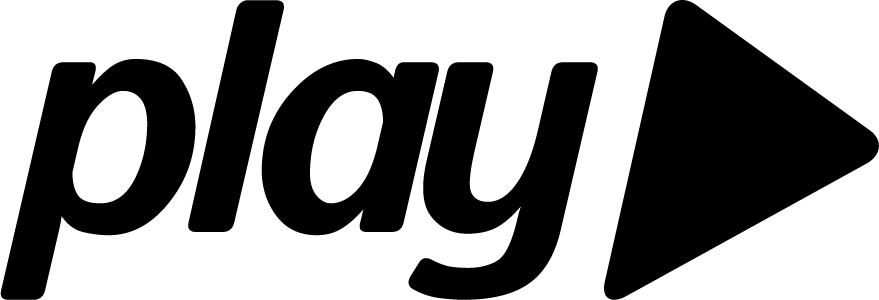
\includegraphics[height=30px]{play.png} %~ ~ 
\includegraphics[height=20px]{backbone.png}
	\\
	\vspace{1cm}
	\normalsize{\today}
}
\titlepage
\end{frame}
}

%%%%%%%%%%%%%%%%%%%%%%%%%%%%%%%%%%%%%%%%%%%%%%%%%%%%%%
%%%%%%%%%%%%%%%%%%%%%%%%%%%%%%%%%%%%%%%%%%%%%%%%%%%%%%

\begin{frame}{Table of Contents}
\tableofcontents[hideallsubsections]
\end{frame}

%%%%%%%%%%%%%%%%%%%%%%%%%%%%%%%%%%%%%%%%%%%%%%%%%%%%%%
%%%%%%%%%%%%%%%%%%%%%%%%%%%%%%%%%%%%%%%%%%%%%%%%%%%%%%

\section{\scshape Introduction}
\subsection{Trends}
\begin{frame}
\frametitle{Trends}
	\begin{itemize}
		\item{Enterprises's needs lead the market.}
		\item{Offering services: SOA wins.}
		\item{The web changes the status quo.}
		\item{SOA is not web compliant.}
		\item{Exposing services through the web requires extra effort.}
		\item{The game changes: new possibilities and challenges.}
	\end{itemize}
\end{frame}

%%%%%%%%%%%%%%%%%%%%%%%%%%%%%%%%%%%%%%%%%%%%%%%%%%%%%%
%%%%%%%%%%%%%%%%%%%%%%%%%%%%%%%%%%%%%%%%%%%%%%%%%%%%%%

\subsection{Challenges}
\begin{frame}
\frametitle{Challenges}
	\begin{itemize}
		\item{Real time data has to be pushed.}
		\item{Huge amounts of data.}
		\item{Need for scalability and integration.}
		\item{Easy integration and accessibility.}
		\item{Interoperability.}
	\end{itemize}
\end{frame}

%%%%%%%%%%%%%%%%%%%%%%%%%%%%%%%%%%%%%%%%%%%%%%%%%%%%%%
%%%%%%%%%%%%%%%%%%%%%%%%%%%%%%%%%%%%%%%%%%%%%%%%%%%%%%

\subsection{Addressing the challenges}
\begin{frame}
\frametitle{Addressing the challenges}
	\begin{itemize}
		\item{Embrace the internet.}
		\begin{itemize}
			\item{HTTP Protocol}
			\item{HTML5}
			\item{XML/JSON}
			\item{Javascript}
			\item{CSS}
		\end{itemize}
		\item{Paradigm shift: client-side.}
		\item{Simplicity.}
		\item{A framework to rule them all.}
		\item{\Large{\textbf{Patterns for enterprise applications}.}}
	\end{itemize}
\end{frame}

%%%%%%%%%%%%%%%%%%%%%%%%%%%%%%%%%%%%%%%%%%%%%%%%%%%%%%
%%%%%%%%%%%%%%%%%%%%%%%%%%%%%%%%%%%%%%%%%%%%%%%%%%%%%%

\section{\scshape Play! Framework}
\subsection{What is Play! Framework?}
\begin{frame}{What is Play! Framework?}
	\begin{itemize}
		\item{A web framework focused on:}
		\begin{itemize}
			\item{Simplicity.}
			\item{Productivity.}
			\item{Scalability.}
			\item{Designed for the modern web.}
			\begin{itemize}
				\item{Concentrate on server-side.}
				\item{Delegate AMAP to the client.}
			\end{itemize}
			\item{Embrace internet standards.}
			\item{Java and Scala.}
			\item{RESTful architecture web applications.}
			\item{Model-View-Controller.}
		\end{itemize}
	\end{itemize}
\end{frame}

%%%%%%%%%%%%%%%%%%%%%%%%%%%%%%%%%%%%%%%%%%%%%%%%%%%%%%
%%%%%%%%%%%%%%%%%%%%%%%%%%%%%%%%%%%%%%%%%%%%%%%%%%%%%%

\subsection{RESTful Architecture}
\begin{frame}{RESTful architecture}
	\begin{itemize}
		\item{Implemented using HTTP and REST principles.}
		\item{Representational state transfer (REST) principles:}
		\begin{itemize}
			\item{Uniform interface.}
			\item{Stateless.}
			\item{Caching.}
			\item{Layers.}
			\item{Code on demand.}
		\end{itemize}
		\item{Goals:}
		\begin{itemize}
			\item{Performance.}
			\item{Scalability.}
			\item{Portability.}
			\item{Reliability.}
			\item{SIMPLICITY.}
		\end{itemize}
	\end{itemize}
\end{frame}

%%%%%%%%%%%%%%%%%%%%%%%%%%%%%%%%%%%%%%%%%%%%%%%%%%%%%%
%%%%%%%%%%%%%%%%%%%%%%%%%%%%%%%%%%%%%%%%%%%%%%%%%%%%%%

\subsection{Project layout}
\begin{frame}{Project layout}
	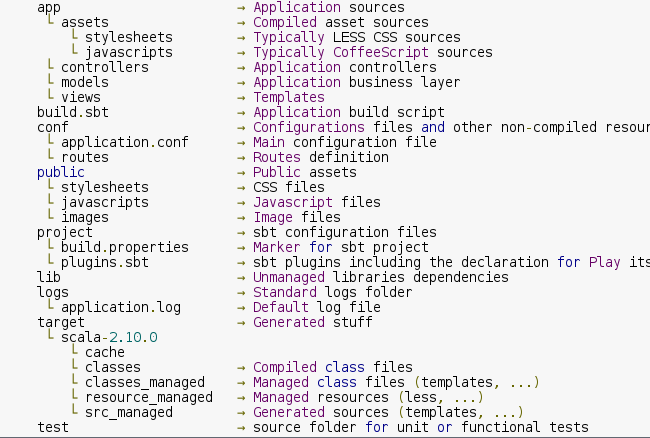
\includegraphics[height=200px]{layout.png}
\end{frame}


%%%%%%%%%%%%%%%%%%%%%%%%%%%%%%%%%%%%%%%%%%%%%%%%%%%%%%
%%%%%%%%%%%%%%%%%%%%%%%%%%%%%%%%%%%%%%%%%%%%%%%%%%%%%%

\section{\scshape Patterns in Play!}

%%%%%%%%%%%%%%%%%%%%%%%%%%%%%%%%%%%%%%%%%%%%%%%%%%%%%%
%%%%%%%%%%%%%%%%%%%%%%%%%%%%%%%%%%%%%%%%%%%%%%%%%%%%%%

\subsection{Model-View-Controller}
\subsubsection{The MVC application model: Models}
\begin{frame}{The MVC application model}
	\begin{itemize}
		\item{Models in app/models}
		\begin{itemize}
			\item{Java/Scala classes.}
			\item{Data + Operations, mainly object-oriented.}
			\item{Business logic and storage.}
		\end{itemize}
	\end{itemize}
\end{frame}

\begin{frame}[fragile]{A model example (models/User.java)}
	\lstset{language=Java}
	\begin{lstlisting}
	package models;
	
	@Entity
	public class User extends Model {
	  @Id
	  public String name;
	  @Required
	  public String pass;
		
	  public User (String name, String pass) {
	      this.name 	= name;
	      this.pass 	= pass;
	  }
		
  public static Finder<String, User> find = new Finder<String, User>(String.class, User.class);
		
  public static List<User> all() {
    return find.all();
  }
	}
	\end{lstlisting}
\end{frame}

\begin{frame}{The MVC application model: Views}
	\begin{itemize}
		\item{Views in app/views}
		\begin{itemize}
			\item{HTML/XML/JSON/Scala templates.}
			\item{Directives as placeholders for data.}
			\item{Render models to user interfaces.}
		\end{itemize}
	\end{itemize}
\end{frame}

\begin{frame}[fragile]{A view example (views/index.scala.html)}
	\lstset{language=HTML}
	\begin{lstlisting}
@(title: String, users: List[User])

<!DOCTYPE html>

<html>
    <head>
        <title>Play! Hello world</title>
    </head>
    <body>
      <header>
	        <h1>@title</h1>
      </header>
      
      <section>
        <ul>
          @for(u <- users) {
            <li>@u.name</li>
          } 
        </ul>
      </section>
    </body>
</html>
	\end{lstlisting}
\end{frame}

\begin{frame}{The MVC application model: Controllers}
	\begin{itemize}
		\item{Controllers in app/controllers}
		\begin{itemize}
			\item{Java/Scala classes.}
			\item{Methods as actions, mainly procedural.}
			\item{Receive requests, act (update models + render views) and response.}
		\end{itemize}
	\end{itemize}
\end{frame}

\begin{frame}[fragile]{A controller example (controllers/Application.java)}
	\lstset{language=Java}
	\begin{lstlisting}
package controllers;

import models.User;
import play.*;
import play.data.*;
import play.mvc.*;
import views.html.*;

public class Application extends Controller 
{
    public static Result index() 
    {
        return ok("Hello, world!", index.render(User.all());
    }
}
	\end{lstlisting}
\end{frame}

\subsubsection{Request/Response path}
\begin{frame}{Request/Response flow}
	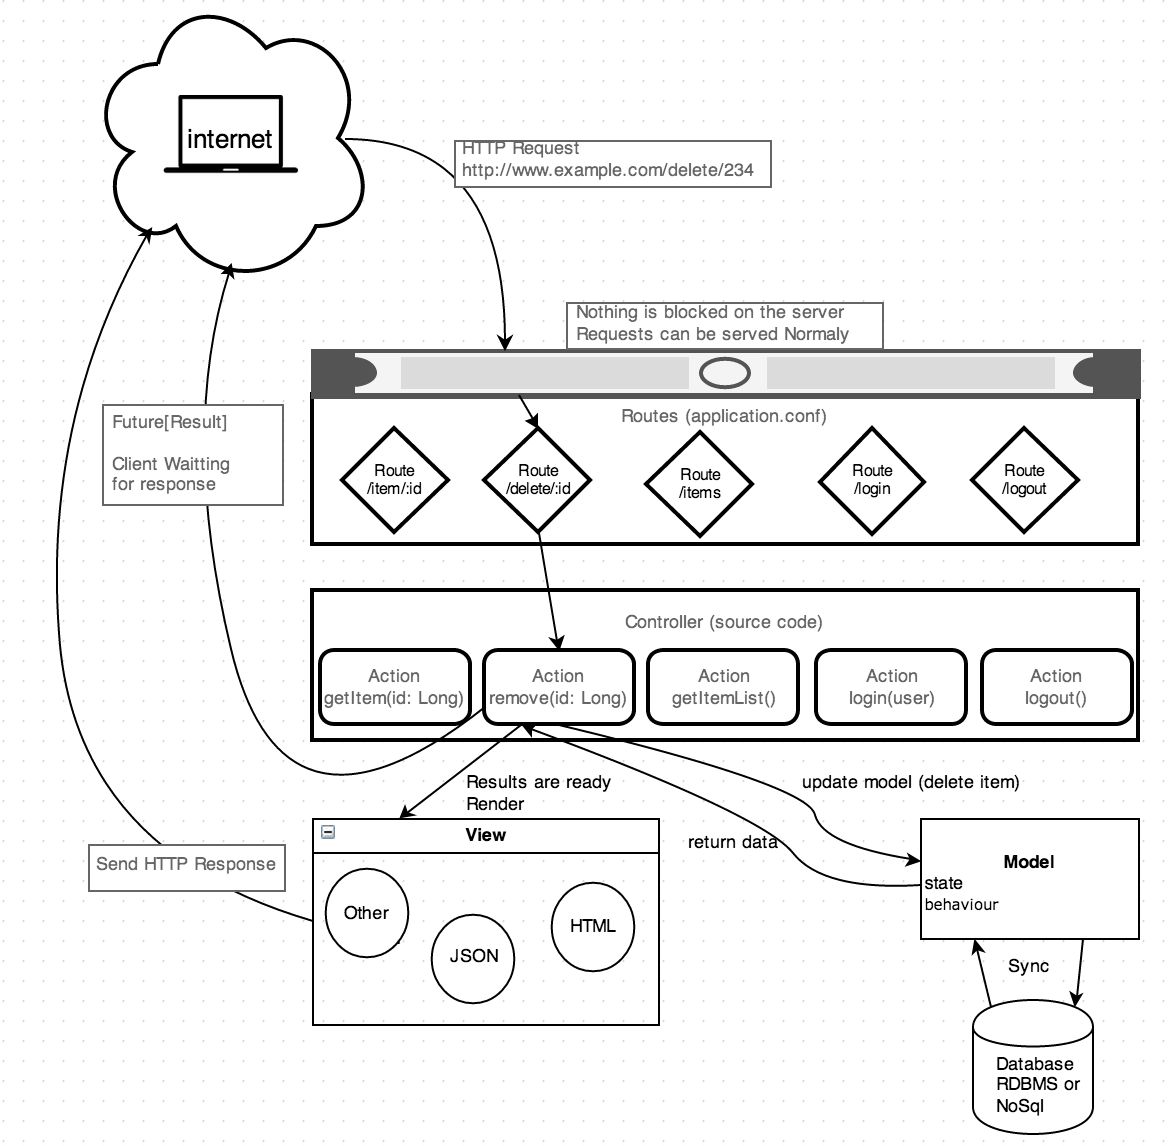
\includegraphics[height=270px]{playarch.png}
\end{frame}

\begin{frame}[fragile]{The HTTP Request and the router (Example)}
	\begin{itemize}
		\item{Suppose that we receive the HTTP Request: \textbf{GET /}}
		\item{The server processes it, looks for the proper action to response the GET / request in \textbf{conf/routes}.}
		\item{The called action is: \textbf{Application.index()}}
	\end{itemize}
	\lstset{language=Java}
	\begin{lstlisting}
# Routes
# All application routes (Higher priority routes first)
# ~~~~
# Home page
GET     /         controllers.Application.index()

# Login
GET     /login    controllers.Application.login()
POST    /login    controllers.Application.authenticate()

#Logout
GET     /logout   controllers.Application.logout()

	\end{lstlisting}
\end{frame}

\begin{frame}[fragile]{A controller example (controllers/Application.java)}
	\lstset{language=Java}
	\begin{lstlisting}
package controllers;

import models.User;
import play.*;
import play.data.*;
import play.mvc.*;
import views.html.*;

public class Application extends Controller 
{
    public static Result index() 
    {
        return ok(index.render("Hello, world!", User.all());
    }
}
	\end{lstlisting}
\end{frame}


\begin{frame}[fragile]{A model example (models/User.java)}
	\lstset{language=Java}
	\begin{lstlisting}
	package models;
	
	@Entity
	public class User extends Model {
	  @Id
	  public String name;
	  @Required
	  public String pass;
		
	  public User (String name, String pass) {
	      this.name 	= name;
	      this.pass 	= pass;
	  }
		
  public static Finder<String, User> find = new Finder<String, User>(String.class, User.class);
		
  public static List<User> all() {
    return find.all();
  }
	}
	\end{lstlisting}
\end{frame}

\begin{frame}[fragile]{A view example (views/index.scala.html)}
	\lstset{language=HTML}
	\begin{lstlisting}
@(title: String, users: List[User])

<!DOCTYPE html>

<html>
    <head>
        <title>Play! Hello world</title>
    </head>
    <body>
      <header>
	        <h1>@title</h1>
      </header>
      
      <section>
        <ul>
          @for(u <- users) {
            <li>@u.name</li>
          } 
        </ul>
      </section>
    </body>
</html>
	\end{lstlisting}
\end{frame}

\begin{frame}[fragile]{The end result}
	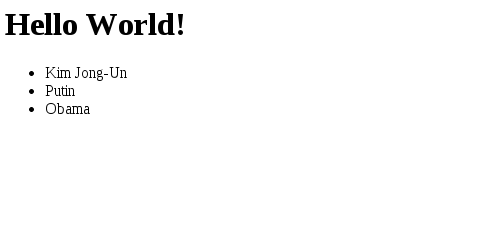
\includegraphics[height=140px]{result.png}
\end{frame}

%%%%%%%%%%%%%%%%%%%%%%%%%%%%%%%%%%%%%%%%%%%%%%%%%%%%%%
%%%%%%%%%%%%%%%%%%%%%%%%%%%%%%%%%%%%%%%%%%%%%%%%%%%%%%


%%%%%%%%%%%%%%%%%%%%%%%%%%%%%%%%%%%%%%%%%%%%%%%%%%%%%%
%%%%%%%%%%%%%%%%%%%%%%%%%%%%%%%%%%%%%%%%%%%%%%%%%%%%%%

\subsection{Model}
\subsubsection{Object Relational Mapping}
\begin{frame}{Object Relational Mapping}
	\begin{itemize}
		\item{Need for persistence (objects outlive the application).}
		\item{Persistence by means of a database.}
		\begin{itemize}
			\item{\textbf{Relational} (RDBMS)}
			\item{Object (ODBMS)}
		\end{itemize}
		\item{Gap between domain model and the relational database.}
		\item{The Object-Relational impedance mismatch.}
		\begin{itemize}
			\item{Granularity}
			\item{Inheritance}
			\item{Identity}
			\item{Associations}
			\item{Data navigation}
		\end{itemize}
		\item{Logical representation to atomized one to store in a DB.}
		\end{itemize}
\end{frame}

\begin{frame}{Object Relational Mapping tools}
	\begin{itemize}
		\item{Object Relational Mapping tools are a possible solution.}
		\item{Provide simple ways to determine the mapping.}
		\begin{itemize}
			\item{XML configuration files.}
			\item{Annotations in the classes.}
		\end{itemize}
		\item{Provide data query and retrieval facilities.}
		\item{All that glitters is not gold...}
		\begin{itemize}
			\item{Pros: Simplicity, dramatically decrease the amount of code.}
			\item{Cons: Higher abstraction drawbacks...}
			\begin{itemize}
				\item{Performance issues.}
				\item{Poor database design.}
			\end{itemize}
		\end{itemize}
		\item{Play! uses Ebean as its ORM of choice.}
	\end{itemize}
\end{frame}

\begin{frame}[fragile]{ORM: Annotated Java model}
\lstset{language=Java}
	\begin{lstlisting}
	package models;
	 
	@Entity
	public class Post extends Model {
	 
	 	@Id
	 	public Long id;
	 	
	 	@Constraints.Required
	    public String title;
	    
	    @Formats.DateTime(pattern="dd/MM/yyyy")
	    public Date postedAt;
	    
	    public String content;
	    
	    @ManyToOne
	    public User author;
	    
	    @OneToMany(mappedBy="post", cascade=CascadeType.ALL)
	    public List<Comment> comments;
	}
	\end{lstlisting}
\end{frame}

\begin{frame}[fragile]{ORM: Usage}
\begin{lstlisting}
		User user = new User("test@test.com", "Test", "test");
		user.save();
		
		User user = User.find.where().eq("email", "test@test.com").findUnique();
		
		User.find.ref("test@test.com").delete();
\end{lstlisting}

ORM Hate by Martin Fowler \cite{ORMHate}
\end{frame}

%%%%%%%%%%%%%%%%%%%%%%%%%%%%%%%%%%%%%%%%%%%%%%%%%%%%%%
%%%%%%%%%%%%%%%%%%%%%%%%%%%%%%%%%%%%%%%%%%%%%%%%%%%%%%

\subsection{View}
\subsubsection{Template View}
\begin{frame}{Template View}
	\begin{itemize}
		\item{\begin{quote}
		"Renders information into HTML by embedding markers in an HTML page"\cite{PEAA}
		\end{quote}}
	\end{itemize}
	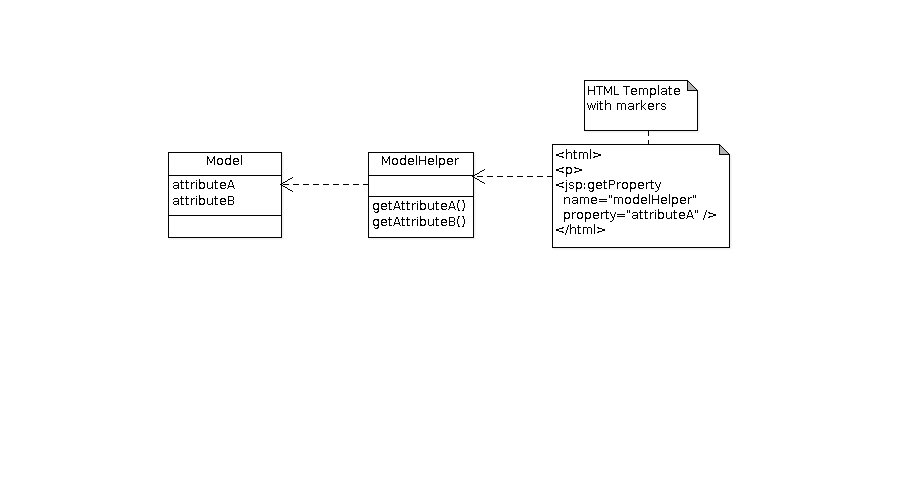
\includegraphics[clip=true,trim={120px 220px 100px 65px},height=110px]{templateview.png}
			\begin{itemize}
				\item{Pros: Lot of power and flexibility in presentation.}
				\item{Cons: Messy code, difficult to maintain, need helpers.}
			\end{itemize}
\end{frame}

\begin{frame}{Template View}
	\begin{itemize}
		\item{\begin{quote}
		The template with annotations is compiled to a Scala.class with a render() method with the template parameters.
		\end{quote}}
	\end{itemize}
	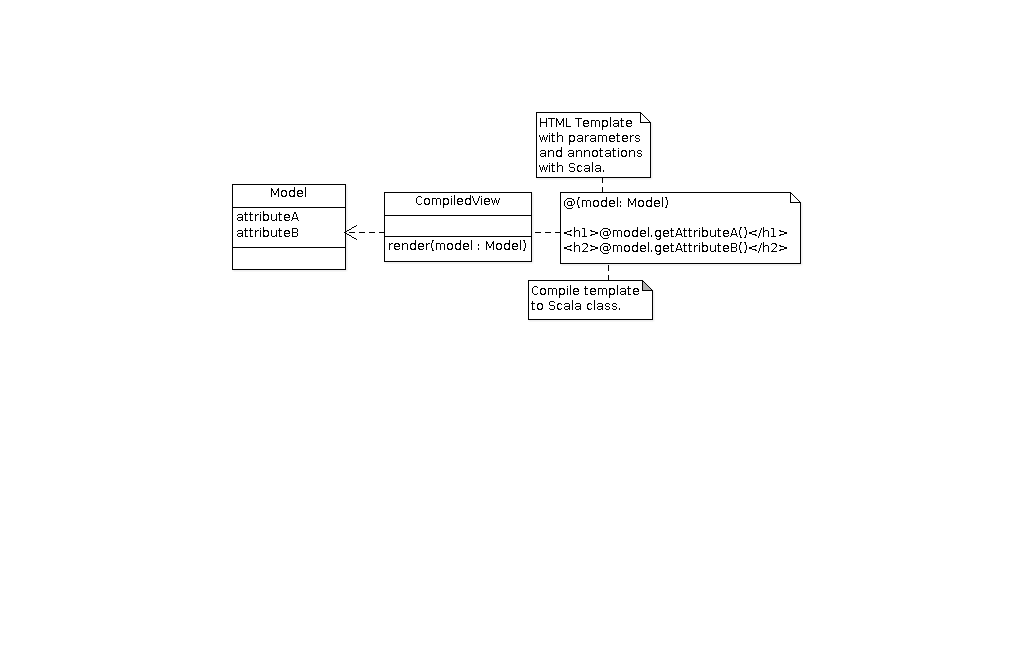
\includegraphics[clip=true,trim={200px 350px 100px 110px},height=110px]{templateviewplay.png}
			\begin{itemize}
				\item{The controller calls the render method of the view.}
				\item{The view communicates with the model (parameter).}
			\end{itemize}
\end{frame}

\begin{frame}[fragile]{Template View example}
	\lstset{language=HTML}
	\begin{lstlisting}
@(title: String, users: List[User])

<!DOCTYPE html>

<html>
    <head>
        <title>Play! Hello world</title>
    </head>
    <body>
      <header>
	        <h1>@title</h1>
      </header>
      
      <section>
        <ul>
          @for(u <- users) {
            <li>@u.name</li>
          } 
        </ul>
      </section>
    </body>
</html>
	\end{lstlisting}
\end{frame}

%%%%%%%%%%%%%%%%%%%%%%%%%%%%%%%%%%%%%%%%%%%%%%%%%%%%%%
%%%%%%%%%%%%%%%%%%%%%%%%%%%%%%%%%%%%%%%%%%%%%%%%%%%%%%

\subsubsection{Composite View}
\begin{frame}{Composite View}
	\begin{itemize}
		\item{\begin{quote}
		A view is built from other views that combine into a composite whole, managing the content and the layout independently.
		\end{quote}}
	\end{itemize}
	\centering
	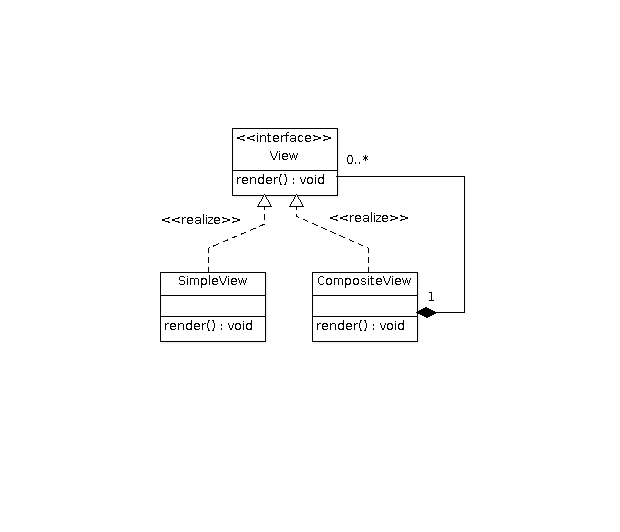
\includegraphics[clip=true,trim={120px 180px 100px 120px},height=110px]{compositeview.png}
			\begin{itemize}
				\item{Pros: Modularity, reuse.}
				\item{Cons: Performance, maintainability.}
			\end{itemize}
\end{frame}

\begin{frame}[fragile]{Composite View}
	\begin{itemize}
		\item{\begin{quote}
		A sample simple view: simpleview.scala.html
		\end{quote}}
		\end{itemize}
		\lstset{language=HTML}
		\begin{lstlisting}
		@(someModel: Model)
		
		@compositeView(someModel) {
		  <header>
		    <hgroup>
		      <h1>Model data</h1>
		      <h2>@someModel.doSomething()</h2>
		    </hgroup>
		  </header>
		}
		\end{lstlisting}
\end{frame}

\begin{frame}[fragile]{Composite View}
	\begin{itemize}
		\item{\begin{quote}
		A composite view: compositeView.scala.html
		\end{quote}}
		\end{itemize}
		\lstset{language=HTML}
		\begin{lstlisting}
@(someModel: Model)(simpleView: Html)
<html>
    <head>
        <title>Composite View Example</title>
    </head>
    <body>
        @simpleView
        
        <section id="main">
        	@someModel.showSomething()
        </section>
    </body>
</html>
		\end{lstlisting}
\end{frame}


%%%%%%%%%%%%%%%%%%%%%%%%%%%%%%%%%%%%%%%%%%%%%%%%%%%%%%
%%%%%%%%%%%%%%%%%%%%%%%%%%%%%%%%%%%%%%%%%%%%%%%%%%%%%%

\subsection{Controller}
\subsubsection{Front Controller}
\begin{frame}{Front Controller Pattern}
	\begin{itemize}
		\item{\begin{quote}
		"Consolidates all request handling by channeling requests through a single handler object" \cite{PEAA}
		\end{quote}}
	\end{itemize}
	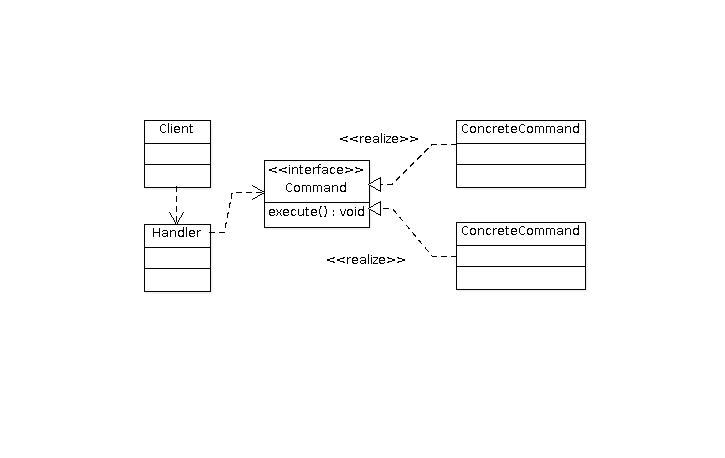
\includegraphics[clip=true,trim={50px 160px 100px 120px},height=90px]{frontcontroller.png}
		\begin{itemize}
			\item{Pros: Centralized control, Thread safety, Configurability.}
			\item{Cons: Possible performance issues, Maintenance costs.}
		\end{itemize}
\end{frame}

\begin{frame}{Front Controller in Play!}
	\begin{itemize}
		\item{The router (handler) selects a controller (command) and a particular action (execute) depeding on the HTTP request.}
	\end{itemize}
	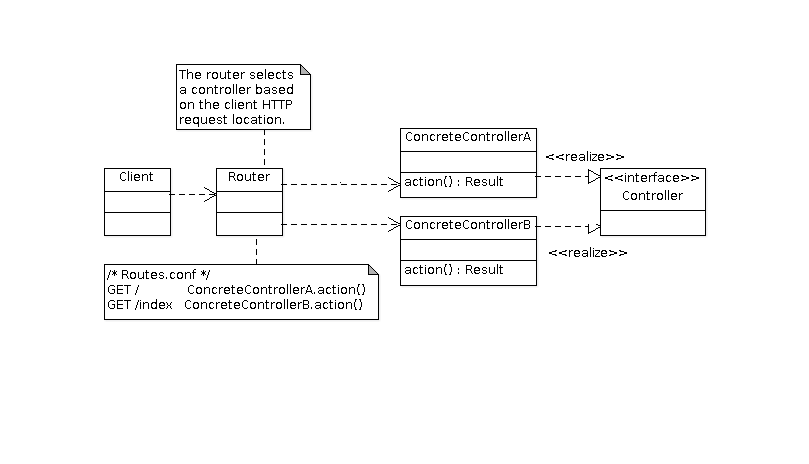
\includegraphics[clip=true,trim={50px 130px 100px 65px},height=120px]{frontcontrollerplay.png}
		\begin{itemize}
			\item{Routes.conf file determines the location-action relationship.}
			\item{Actions return a result that holds the HTTP Response.}
		\end{itemize}
\end{frame}

\begin{frame}[fragile]{The Router}
	\begin{itemize}
		\item{The conf/routes file is compiled to a Router class.}
	\end{itemize}
	\lstset{language=Java}
	\begin{lstlisting}
# Routes
# All application routes (Higher priority routes first)
# ~~~~
# Home page
GET     /         controllers.Application.index()

# Login
GET     /login    controllers.Application.login()
POST    /login    controllers.Application.authenticate()

#Logout
GET     /logout   controllers.Application.logout()

	\end{lstlisting}
\end{frame}

%%%%%%%%%%%%%%%%%%%%%%%%%%%%%%%%%%%%%%%%%%%%%%%%%%%%%%
%%%%%%%%%%%%%%%%%%%%%%%%%%%%%%%%%%%%%%%%%%%%%%%%%%%%%%

\section{\scshape Conclusions}
\begin{frame}
	\begin{itemize}
		\item{Web programming is evolving (again).}
		\begin{itemize}
			\item{Scalability.}
			\item{Client-side.}
			\item{Frameworks to deal with complexity.}
		\end{itemize}
		\item{Patterns are not just theoretical models.}
		\begin{itemize}
			\item{Applied in modern applications.}
			\item{Guides, not fixed templates.}
			\item{With great power, comes great responsibility.}
		\end{itemize}
		\item{Play! applies patterns for modern applications.}
		\begin{itemize}
			\item{Easy learning curve.}
			\item{Deep enough for complex applications.}
			\item{Supported by Typesafe (Scala creators).}
			\item{Not perfect.}
			\begin{itemize}
				\item{Difficult upgrades.}
				\item{Documentation is not so great.}
				\item{Not the most popular.}
			\end{itemize}
		\end{itemize}
	\end{itemize}
\end{frame}

%%%%%%%%%%%%%%%%%%%%%%%%%%%%%%%%%%%%%%%%%%%%%%%%%%%%%%
%%%%%%%%%%%%%%%%%%%%%%%%%%%%%%%%%%%%%%%%%%%%%%%%%%%%%%

\section*{\scshape References}
\begin{frame}
	\normalsize
	\nocite{PlayForJava}
	\nocite{PlayForScala}
	\nocite{PlayFrameworkCookbook}
	\frametitle{References}
	\bibliographystyle{amsalpha}
	\bibliography{biblio}
\end{frame}

\end{document}